\documentclass{article} % For LaTeX2e
\usepackage{iclr2027_conference,times}

\input{math_commands.tex}

\usepackage{hyperref}
\usepackage{url}
\usepackage{booktabs}
\usepackage{multirow}
\usepackage{amsmath,amssymb,amsthm}
\usepackage{graphicx}

\newtheorem{proposition}{Proposition}
\newtheorem{lemma}{Lemma}

% Uncomment for camera-ready
%\iclrfinalcopy

\title{GoldiMask: Fine-Tuning Diffusion Language Models\\in the Measured Zone of Learnability}

\author{Anonymous authors\\
Paper under double-blind review}

\newcommand{\fix}{\marginpar{FIX}}
\newcommand{\new}{\marginpar{NEW}}

\begin{document}

\maketitle

\begin{abstract}
Every training step of a masked diffusion language model makes a decision that is usually left to chance: which tokens of the target are visible as context, and which remain masked and supervised. Recent work (LIFT) showed that making this decision by model confidence improves supervised fine-tuning. We go further and ask what the decision \emph{should} be---and instead of designing an answer, we measure it. Two cheap diagnostics (roughly twenty-five GPU-minutes each, run on the base model) yield two stable empirical regularities: a \emph{learnability curve}, showing that the benefit of teaching a token peaks when the model assigns it probability $\approx 0.22$, regardless of noise level; and a \emph{support curve}, showing that revealed context helps a masked token in proportion to the attention it directs at that context, with gentle saturation. From these two curves we derive GoldiMask, a corruption-design objective that reveals the tokens whose visibility delivers the most predicted learning to the tokens worth teaching, together with a loss weighting by each token's \emph{realized} learning. The objective is submodular, its opportunity cost is built in, and the attention-based selection heuristics we first hand-designed emerge as its limiting cases. A randomized control decomposes the total gain: roughly half comes from the two-pass reveal structure itself and half from what is revealed --- a separation no prior corruption-design work provides. Fine-tuning LLaDA-8B on the s1K dataset under LIFT's protocol, GoldiMask raises the four-benchmark core average from $39.5 \pm 0.4$ (LIFT) to $41.0 \pm 0.8$ over three seeds, with no seed overlap; transplanted unchanged---same curves, same hyperparameters---to Dream-7B it exceeds the strongest published configuration by $1.4$--$1.8$ points ($45.1 \pm 1.6$ versus $43.7$), and on the harder 12K corpus it matches the best published variant with no per-dataset tuning. A sampling-temperature analysis attributes the remaining AIME gap to distributional sharpening rather than missing knowledge: at matched elevated temperature the two methods' summed AIME tails are statistically indistinguishable, and the sharper model gains more from temperature, as the account predicts. A default-parameter variant retains the full gain, so deployment requires no calibration at all: the measurements justify the shape of the method, and the shape is all that matters---controls trained with deliberately wrong-shaped learnability curves lose the gain in proportion to how far their peak sits from the measured one, the worst collapsing to the random-reveal floor.
\end{abstract}

\section{Introduction}

Masked diffusion language models learn by filling in blanks. During supervised fine-tuning, a target response is corrupted---each token independently masked with some probability---and the model is trained to reconstruct the masked tokens from the visible remainder. The corruption is almost always random. This is a curious convention, because the corruption defines the entire learning problem of that step: the visible tokens are the lesson's material, the masked tokens are its exercises, and a random split has no reason to be a good lesson.

LIFT \citep{lift2026} and GIFT \citep{gift2025} were the first to treat this split as a design space for diffusion-LM fine-tuning; GIFT assigns per-token masking rates from entropy, while LIFT --- whose two-pass structure we build on --- ranks masked tokens by model confidence and supervises either the most or the least confident ones depending on the noise level, revealing the rest. The gains are real, and we reproduce them. But confidence ranking answers only half of the question, and answers it indirectly. The full question has two parts: which tokens are \emph{worth teaching} right now, and which visible context would \emph{most help} teach them. Confidence is a proxy for the first part and silent on the second.

Our starting point is that both parts can be estimated far more directly than confidence ranks allow. (Directly is not perfectly: our learnability estimate is itself a proxy for training benefit --- but one built from a randomized, per-token contrast rather than a static score, and validated out of sample.) The two-pass structure that LIFT already uses---a gradient-free forward pass before the supervised one---produces, for free, everything needed to measure them. Masking the same text at two nested corruption levels and comparing the gold token's probability tells us how much a token actually benefits from added context; doing this over a million tokens of training data yields what we call the \emph{learnability curve} $\lambda(p, t)$: the expected benefit of teaching a token, as a function of the model's current probability $p$ for it and the noise level $t$. The curve has a shape that no common heuristic anticipates. Under the standard residual-difficulty valuation (gain weighted by $1-p$), it is a lopsided inverted U whose peak sits at $p \approx 0.22$ in every noise regime we measured; the raw, unweighted context gain peaks higher (at $p \approx 0.5$--$0.8$), and its robust qualitative content is that gain collapses as $p \to 0$: hopeless tokens are not helped by context, which alone rules out the pessimistic $1-p$ weighting. Weighting schemes of the form $1-p$ (pessimism) or $p(1-p)$ (symmetric uncertainty) both miss this shape, one at each end.

A second experiment measures the other half of the question. Holding the supervised tokens fixed and randomizing \emph{which} other tokens are revealed, we find that a masked token's prediction improves in proportion to the attention it directs at the revealed set---the \emph{support curve} $\phi$---rising monotonically with gentle saturation. The saturation matters: it says a token needs enough support, not all the support, which is precisely the regime between the two failure modes we observe empirically (concentrating all reveals on global hubs, and spreading them thin for coverage).

With both curves in hand, the method almost writes itself. Reveal the set $R$ of tokens that maximizes the predicted learning delivered to the tokens that remain masked,
\[
F(R) \;=\; \sum_{i \notin R} \lambda(p_i, t)\, \phi\!\big(S_i(R)\big),
\qquad S_i(R) = \sum_{j \in R} A_{ij},
\]
where $A$ is the model's own attention; then weight each supervised token's loss by its \emph{realized} learning, the measured improvement the revealed context actually produced, discounted by the same curve. One quantity---learnability transfer---is used prospectively to construct the corruption and retrospectively to allocate the gradient. The objective turns out to have pleasant structure: it is submodular for any concave $\phi$ (a short proof), its opportunity cost is endogenous---revealing a token deletes that token's own term, so the optimizer never sacrifices a teachable token to make a hint---and with a linear $\phi$ and uniform $\lambda$ it collapses to the incoming-attention heuristic that was our strongest hand-designed baseline. The heuristic, it turns out, was the first-order approximation of the measurement.

We call the method GoldiMask, after the zone the learnability curve locates: not too easy, not too hard. The name is more than decoration. The framework that organizes all of our findings is the classroom: $\lambda$ locates each token's zone of proximal development; the reveal set is scaffolding, built from material that is either already mastered or currently beyond reach --- and therefore cheap to give away; the realized-gain weighting is assessment, spending practice where progress is demonstrated; and---as our analysis of the AIME benchmark shows---scaffolds must eventually be faded, because a model that always trains with helpful context underperforms, at sampling time, on exams that begin from a blank page. Each of these classroom intuitions appears in our experiments as a measured effect rather than a design choice.

Our contributions:
\begin{itemize}
\item \textbf{Two measurement protocols} for masked-diffusion fine-tuning, each costing about twenty-five GPU-minutes: nested-corruption probing for the learnability curve, and fixed-target reveal randomization for the support curve. Both estimates come from within-token randomized contrasts (with the dose--response additionally assuming attention support mediates the reveal-set effect), are stable under split-half validation ($r = 0.97$), and robust to $2\times$ parameter perturbation (rank correlation $\geq 0.92$).
\item \textbf{A corruption-design objective} built from the two curves, with a submodularity guarantee, endogenous opportunity cost, and prior heuristics as limiting cases; plus a realized-gain loss weighting that closes the loop.
\item \textbf{Results.} On s1K with LLaDA-8B-Instruct over three seeds, GoldiMask improves the four-benchmark core average from LIFT's $39.5 \pm 0.4$ to $41.0 \pm 0.8$, with no seed overlap (on LIFT's own reported seed: $40.0 \to 41.8$). Transplanted unchanged, it gains $1.4$--$1.8$ points over the strongest published Dream-7B configuration (three seeds) and matches the best published variant on the 12K corpus at equal step budget; individual configurations set per-benchmark highs on GSM8K (82.0, tilt variant), MATH500 (40.4, full fading), and Sudoku (17.5, tilt; each seed 42). A sampling-temperature analysis attributes the remaining AIME gap to distributional sharpening rather than missing knowledge---the fitted variant's average per-attempt solve rate matches LIFT's---and at matched elevated temperature the two methods' summed AIME tails are statistically indistinguishable.
\item \textbf{Ablations that close the obvious objections.} A random-reveal control isolates the causal value of attention-guided selection ($+2$ core points) from the two-pass structure itself (also $+2$ over vanilla SFT). A defaults-only variant, with the fitted curves replaced by round numbers of the right shape, retains the full gain---so the method requires no per-setup calibration; the measurements are the science, not the runtime dependency. Closing the loop, two controls with deliberately wrong-shaped $\lambda$ (peak moved to $p \approx 0.53$ and $p \approx 0.01$; the measured peak is $\approx 0.22$) lose $1.3$ and $3.2$ core points respectively---monotone in how far the peak moves---with the worst collapsing to the random-reveal floor while reproducing the core-versus-tail trade-off from the curve shape alone.
\end{itemize}

We are explicit about scope. The main comparisons---LIFT ($H{=}3$), GoldiMask defaults, the full fading variant, and the Dream-7B, LLaDA-1.5, and 12K transplants---are three seeds each, reported mean $\pm$ sample standard deviation; the remaining variants and the ablations are single-seed (seed 42, the seed the LIFT authors also report individually). We quantify AIME's resolution explicitly (one question is 3.3 points), note that binomial noise on the core benchmarks spans roughly $\pm 1$--$2$ points at their test-set sizes, and mark ties accordingly.

\section{Related Work}

\paragraph{Diffusion language models.} Masked (absorbing-state) discrete diffusion has emerged as a competitive alternative to autoregressive language modeling \citep{austin2021structured,lou2024discrete,sahoo2024simple}. LLaDA \citep{nie2024llada} scaled the recipe to 8B parameters and instruction tuning; LLaDA-1.5 \citep{zhu2025llada15} added preference optimization, and Dream-7B \citep{ye2025dream} adapted a pretrained autoregressive backbone. Our experiments build on LLaDA-8B-Instruct and use the training and evaluation protocol of \citet{lift2026} throughout.

\paragraph{Corruption design for diffusion SFT.} LIFT \citep{lift2026} selects which masked tokens to supervise by confidence rank, with a noise-level-dependent schedule; GIFT \citep{gift2025} gives each token its own masking rate derived from entropy; context-adaptive reweighting (CART, as reported by \citet{lift2026}) weights masked tokens by proximity to visible context. All three act on a proxy---confidence, entropy, or position. Our method differs in that the quantity it optimizes, learnability transfer, is measured directly, and in that it designs the \emph{revealed} set rather than the supervised one: in a fixed-budget corruption these are complementary choices, and we find the reveal side is where attention structure carries information that confidence cannot (the two are nearly uncorrelated in our measurements).

\paragraph{Trajectory- and order-based approaches.} Two recent lines share our premise that the visibility structure of masked-diffusion training and inference is not neutral, while acting on different levers. TABOM \citep{chen2026tabom} post-trains on the model's own decoding trajectories with an entropy-ranking loss, replacing random masks with self-distilled easy-first states; its diagnosis---the mismatch between randomly-masked training and easy-to-hard inference---is the same phenomenon our tail analysis measures (Section~\ref{sec:aime}), reached independently. Our approach differs in both halves: visible sets are chosen by maximizing \emph{measured} learnability transfer rather than replaying decode heuristics (and our random-reveal control shows the selection itself, not merely structured corruption, carries the gain), and our loss reweights by within-step realized improvement rather than aligning certainty orderings. Where-to-Unmask \citep{asano2026unmask} learns an inference-time unmasking planner over a frozen token model---complementary to training-time corruption design, and a natural composition with GoldiMask-trained models.

\paragraph{Token selection and weighting in autoregressive training.} RHO-LOSS \citep{mindermann2022prioritized} selects training points that are ``learnable, worth learning, and not yet learnt'' --- the closest ancestor of our learnability estimand, at example rather than token granularity and via holdout models rather than within-token contrasts; Rho-1 \citep{lin2024rho} applies the idea at token level with a reference model; focal loss \citep{lin2017focal} down-weights easy examples; even random token-level loss masking has proven consequential, e.g.\ for memorization control \citep{hans2025goldfish}. Corruption design itself predates diffusion LMs: the BERT-era masking-policy literature \citep{levine2021pmi,wettig2023mask} established that \emph{what} you mask changes what is learned, and our protocols can be read as its measurement-driven continuation. Expected-error-reduction active learning \citep{settles2009active} is the classical form of ``teach where predicted improvement is largest.'' These methods share our premise that not all tokens deserve equal gradient, but none has access to the counterfactual our setting provides for free: the same token's probability with and without additional context, in the same step. That counterfactual---not confidence, not entropy---is what our weights are built from.

\paragraph{Curriculum and learnability.} Curriculum learning \citep{bengio2009curriculum}, self-paced learning \citep{kumar2010self}, and learning-progress-driven curricula \citep{graves2017automated} formalize the intuition that training is most effective at intermediate difficulty, an idea with a long pedagogical history \citep{vygotsky1978mind} and direct empirical counterparts in cognition: infants preferentially attend to stimuli of intermediate complexity \citep{kidd2012goldilocks} --- the Goldilocks effect our title borrows --- and optimal training accuracy in simple learners has been argued to sit near 85\% \citep{wilson2019eighty}, an interesting contrast with the much lower peak our token-level curve locates. Our learnability curve is, to our knowledge, the first direct token-level measurement of this ``zone'' in language model fine-tuning, and its stability (the peak does not move with noise level, data half, or model checkpoint) suggests it reflects a property of the learning problem rather than an artifact of the estimator. As a side effect, the randomized-reveal protocol speaks to the attention-interpretability debate \citep{jain2019attention}: here attention is validated not as an explanation but as a predictor of interventional context value.

\paragraph{Submodular selection.} Facility location and coverage objectives are classical tools for subset selection \citep{nemhauser1978analysis,krause2014submodular}. We contribute a variant whose client set is the \emph{complement} of the selected set---revealing a token removes it from the objective's beneficiaries---which we show preserves submodularity for concave response functions while making the selection self-paying. Empirically, our measured response curve falls strictly between the linear and hard-max cases that correspond to the two standard heuristics, and the calibrated middle outperforms both.

\section{Method}

\subsection{Setup}

Let $x_0$ be a prompt--response pair with response length $L$. Masked-diffusion SFT draws a noise level $t \sim \mathcal{U}(0,1)$ and corrupts the response by masking each token independently (we follow LIFT's over-masking variant: mask at rate $t + \rho$ with $\rho \sim \mathcal{U}(0.1, 1{-}t)$, then reveal back down to $K = \lfloor tL \rfloor$ supervised tokens). The loss is the time-scaled cross-entropy $\sum_{i \in \text{masked}} \mathrm{CE}_i / t$, normalized as in \citet{lift2026}; nothing about the objective, optimizer, or data changes in our method. What changes is the answer to two questions the pipeline already poses: which of the over-masked candidates are revealed back as context, and how much each remaining token's error contributes to the gradient.

Both of our answers are computed from the gradient-free first pass that two-pass methods already run. From it we take each candidate's \emph{confidence} $p_i$ (the model's probability of the gold token) and the final-block \emph{attention} $A_{ij}$ from each candidate $i$ to each candidate $j$ (recomputed explicitly from queries and keys, since fused attention kernels never materialize it; head-averaged; diagonal zeroed).

\subsection{Two measurements}
\label{sec:measurements}

\paragraph{The learnability curve.} For 100 held-out training examples and four noise draws each, we corrupt the same 100 examples (drawn from the training set and reserved for measurement) at two nested levels, $t + \rho$ and $t + \rho/2$, using shared uniform variates so the sparser mask is a strict subset of the denser one. For each of the 957{,}563 tokens masked in both, the gold log-probability under each corruption gives the \emph{context gain}---how much the extra revealed tokens helped---and multiplying by the residual-difficulty valuation $(1-p)$ --- an assumed factor, not a measured one --- gives a per-token learnability sample. Averaging within (confidence bin $\times$ noise bin) cells yields $\lambda(p, t)$. We report the raw context-gain curve alongside: it peaks at $p \approx 0.5$--$0.8$, so the familiar $0.22$ peak location is partly placed by the valuation factor; what the measurement itself establishes is the collapse of gain at both extremes, which no monotone weighting reproduces.

The result (Figure~\ref{fig:curves}, left) is a lopsided inverted U. Its peak sits at $p \approx 0.22$ in all five noise bins; only the amplitude changes with $t$. A three-parameter form $\lambda(p) \propto p^a (1-p)^b$ fits each bin with log-domain $R^2$ between $0.93$ and $0.99$. The curve is not an artifact of the fit: refitting on disjoint halves of the examples reproduces cell means at $r = 0.967$ and moves the peak by $0.01$. Two common weighting heuristics fail against it in different ways: $1-p$ keeps weight on hopeless tokens whose measured gain is small, and $p(1-p)$ puts the peak at $0.5$, twice too far right.

\begin{figure}[t]
\centering
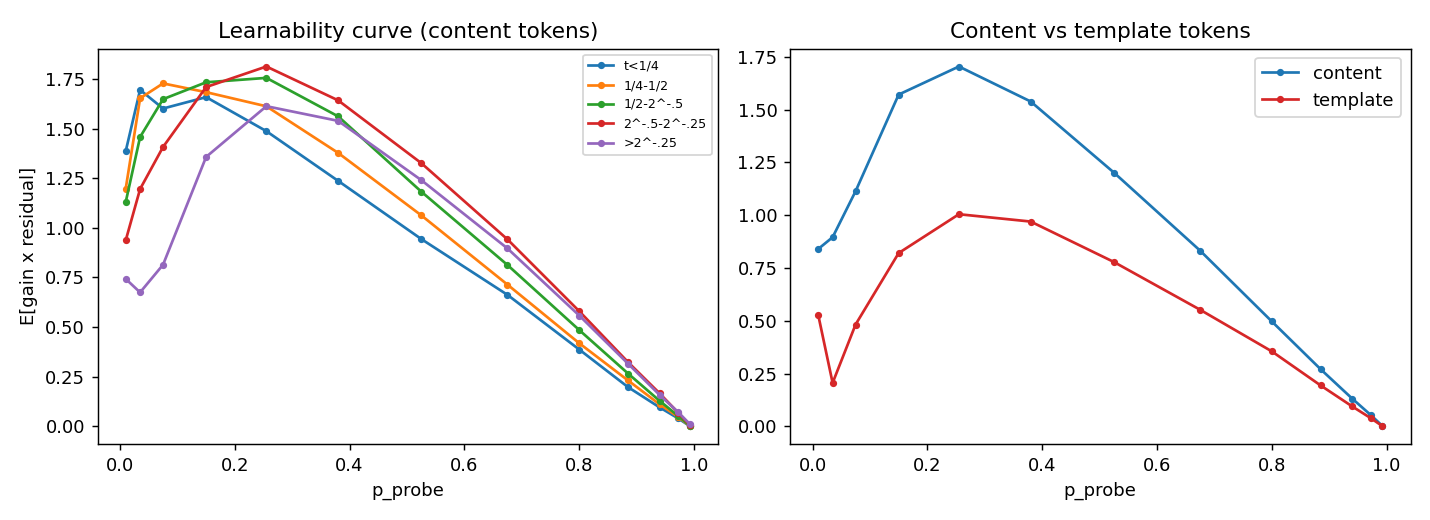
\includegraphics[width=0.86\textwidth]{fig_learnability.png}\\[4pt]
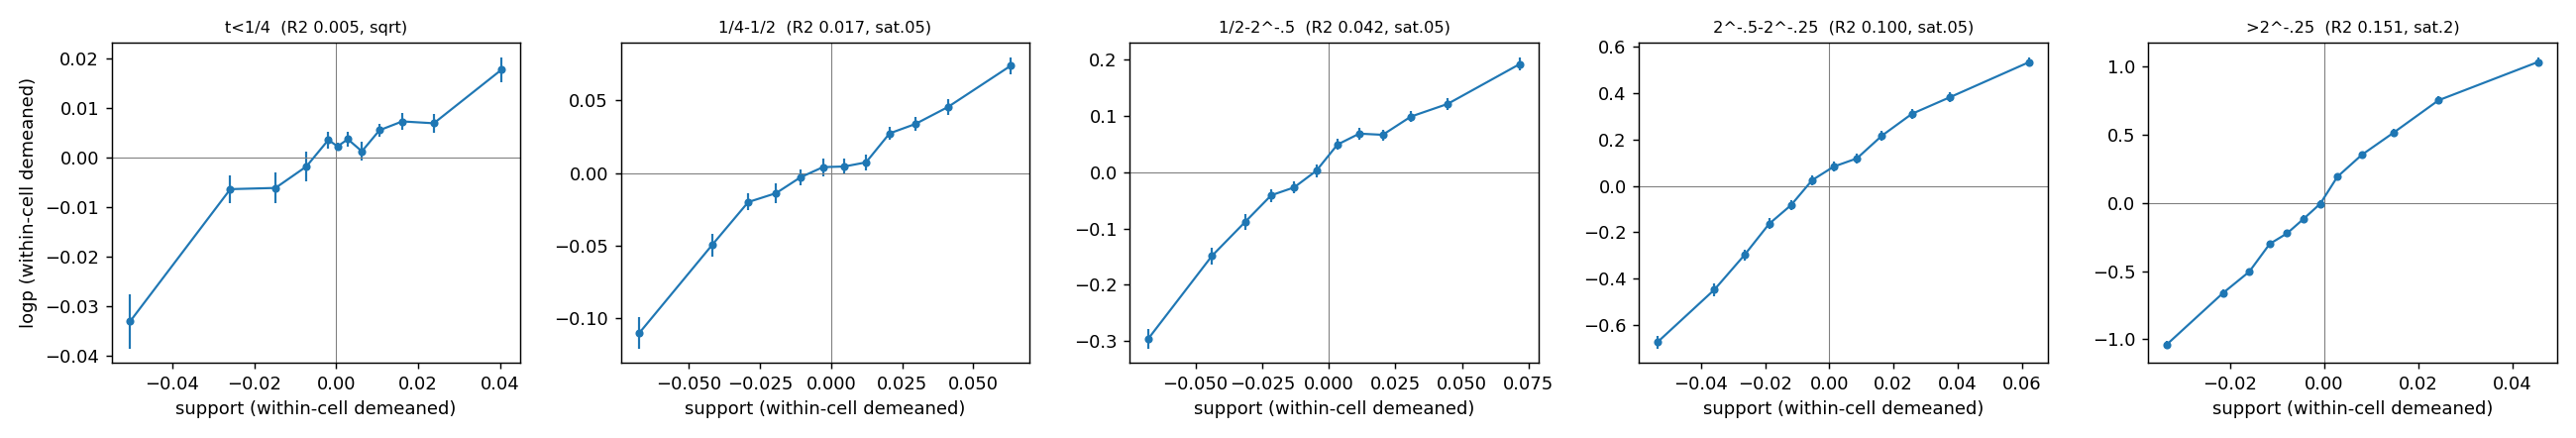
\includegraphics[width=\textwidth]{fig_phi.png}
\caption{\textbf{The two measured curves.} \emph{Top:} the learnability curve $\lambda(p,t)$ over 957{,}563 tokens --- a lopsided inverted U whose peak sits at $p \approx 0.22$ in every noise bin (left), with template tokens carrying little of the mass (right). \emph{Bottom:} the support curve $\phi$ from within-target randomized reveal contrasts (25{,}217 targets $\times$ 8 random sets): monotone in every noise bin, gently saturating, and thirty-fold stronger at high noise --- context identity matters where masking is heavy. Together the two curves fully specify the GoldiMask objective; neither matches any standard hand-designed weighting.}
\label{fig:curves}
\end{figure}

\paragraph{The support curve.} The second protocol asks whether it matters \emph{which} tokens are revealed, holding everything else fixed. For fixed supervised targets, noise level, and reveal budget, we evaluate eight random reveal sets per configuration (25{,}217 targets in total) and record, for each target, its attention mass on each reveal set (the \emph{support} $S_i$) and its resulting gold log-probability. Because only the reveal set varies within a configuration, regressing outcome on support with per-target fixed effects identifies the dose--response $\phi$ under one stated assumption: that attention support is the channel through which reveal-set identity acts (proximity and content overlap are competing mediators we cannot exclude). It is monotone in every noise bin and gently saturating (half-saturation at support $0.05$--$0.2$), and its explanatory power grows thirty-fold from low to high noise---context identity matters where masking is heavy, and hardly at all where it is light. The saturating fit beats a linear one by about twenty percent relative $R^2$ in the decisive bins; a hard-saturation (coverage-style) shape fits worst of all, consistent with coverage-based selection losing to concentration in every head-to-head we ran.

\subsection{The GoldiMask objective}

Given a candidate set $C$ (the over-masked tokens) and a budget $B = |C| - K$ to reveal, choose
\begin{equation}
R^\ast \;=\; \arg\max_{R \subseteq C,\, |R| = B}\; F(R), \qquad
F(R) = \sum_{i \in C \setminus R} \lambda(p_i, t)\,\phi\big(S_i(R)\big), \quad S_i(R) = \sum_{j \in R} A_{ij}.
\label{eq:objective}
\end{equation}
Each still-masked token wants attention support from the revealed set, in proportion to how much it is worth teaching. Three properties make this more than a scoring rule.

\textbf{Submodularity.} For any concave nondecreasing $\phi$ with $\phi(0)=0$ and nonnegative $\lambda, A$, the marginal gain of adding a token to $R$ is nonincreasing in $R$. The proof is three lines from the marginal
\[
\Delta(x \mid R) = \sum_{i \notin R \cup \{x\}} \lambda_i \big[\phi(S_i(R) + A_{ix}) - \phi(S_i(R))\big] \;-\; \lambda_x\, \phi(S_x(R)):
\]
the delivery term shrinks as $R$ grows (fewer clients, higher on a concave curve) and the self-loss term grows in magnitude ($S_x$ increases). The objective is not monotone---revealing a valuable client hurts---but under an exact cardinality budget this costs us nothing operationally, and randomized greedy retains a $1/e$ guarantee \citep{buchbinder2014submodular}. In practice we use chunked greedy with local-search polish; at a few hundred candidates per sequence the whole selection costs about $140$ms per training step, and random restarts confirm the greedy solutions are near-optimal at this scale.

\textbf{Self-paying opportunity cost.} Because the client sum runs over $C \setminus R$, revealing $x$ deletes $x$'s own term: every reveal pays exactly the learnability it forfeits. The optimizer therefore builds context out of tokens that are cheap to give away---already known, or currently hopeless---and protects the mid-confidence band. This single structural property repairs the failure mode we (and, we suspect, others) hit with hand-designed variants, in which difficulty-seeking reveal scores systematically removed the hardest tokens from supervision.

\textbf{Prior heuristics as limits.} With $\phi$ linear and $\lambda$ uniform, greedy selection reduces to ranking candidates by incoming attention from the remaining masked set---within a correction term, exactly the ``reveal the attention hubs'' heuristic that is our strongest hand-designed baseline. The hard-saturation limit of $\phi$ yields weighted coverage (the per-edge max aggregator of facility location is not a limit of additive support; we evaluate coverage-style selection directly). The measured $\phi$ lies strictly between, and at inference time the calibrated middle beats both limits on paired reveal-set comparisons over fixed targets ($+0.107$ nats over the hub heuristic at high noise, bootstrap CI $[+0.069, +0.151]$); after training, it matches the hub heuristic on the core average (a tie under our convention) while adding the checkpoint stability and per-benchmark gains of Section~\ref{sec:experiments}.

\subsection{Closing the loop: realized-gain weighting}

Selection uses \emph{predicted} learning; the loss weighting uses \emph{realized} learning. After the second (supervised) pass, each still-masked token has two probabilities for its gold label: $p_1$ from the heavily-masked first pass and $p_2$ after the chosen context was revealed. We weight token $i$'s cross-entropy by
\begin{equation}
w_i \;\propto\; \max(\log p_2^{(i)} - \log p_1^{(i)},\, 0) \cdot \lambda(p_2^{(i)}, t),
\end{equation}
mean-normalized and capped at $10\times$ (template and formatting tokens occasionally exhibit enormous nominal gains; the cap and the $\lambda$ factor both suppress them). The gain factor credits tokens the scaffolding demonstrably helped; the $\lambda$ factor spends that credit only where more teaching is worthwhile. One quantity, used twice: predicted to build the corruption, measured to allocate the gradient.

\subsection{Instantiations}
\label{sec:instantiations}

\textbf{Fitted vs.\ defaults.} The fitted instantiation uses the measured lookup tables for $\lambda$ and $\phi$ (the submodularity guarantee applies when $\phi$ is projected onto a concave nondecreasing family; the raw binned curve need not be). The \emph{defaults} instantiation replaces them with round numbers of the right shape---$\lambda(p) \propto p(1-p)^3$ (peak $0.25$) and $\phi(s) = s/(s+0.1)$---and, as Section~\ref{sec:ablations} shows, loses nothing. We recommend the defaults in practice and view the measurements as the evidence that licenses them.

\textbf{Fading variants.} A model that always trains with helpfully-chosen context can become dependent on it. We evaluate three ways of mixing in scaffold-free steps, all as stochastic per-step mode choices in the spirit of LIFT's own mode mixture: a \emph{vanilla hedge} (full supervision, no reveal, probability $\propto t(1-t)$), a \emph{noise tilt} (importance-sampling $t$ toward heavy masking, where Section~\ref{sec:measurements} shows selection has leverage, with exact importance-weight correction), and LIFT's own bottom-$k$ hard-token mode (probability $\propto 1-t$). These matter specifically for sampled, from-scratch generation benchmarks, as the next section shows.

\section{Experiments}
\label{sec:experiments}

\subsection{Protocol}

We follow \citet{lift2026} exactly: LLaDA-8B-Instruct fine-tuned on s1K \citep{muennighoff2025s1} with LoRA ($r{=}128$), global batch 8, 20 epochs (2{,}480 steps), evaluated on GSM8K, MATH500, Countdown, and Sudoku at generation lengths $\{128, 256, 512\}$ (best reported, greedy), and on AIME'24/'25 by pass@16 over 16 sampled runs. Main comparisons are three seeds (42--44), reported mean $\pm$ sample standard deviation; single-seed rows are seed 42, and every method sees identical data order within a seed. Multi-seed rows are reported at the checkpoint the original pipeline's selector chooses (its validation-loss rule, applied identically to every method); because we found benchmark scores swing by $\pm 3$ points with checkpoint choice under that selector, we also evaluate the final checkpoint of every run and report both (Table~\ref{tab:main} carries a final-checkpoint core column; the full grid is Appendix~\ref{app:full}); we treat core differences under $1$ point and AIME differences under $2$ questions ($6.7$) as ties throughout. LIFT's $H$ denotes the number of noise-regime modes in its selection mixture ($H{=}3$ adds full-supervision steps to $H{=}2$'s top-$k$/bottom-$k$ pair). Our reproduction of the paper's Table~1 is in Appendix~\ref{app:repro}; the base model matches to the decimal on AIME, and LIFT's orderings replicate.

\subsection{Main results}

\begin{table}[t]
\caption{Core benchmarks (pass@1, greedy, best generation length) and AIME (pass@16), LLaDA-8B-Instruct on s1K. Rows marked $\pm$ are mean $\pm$ sd over seeds 42--44 at the original selector's checkpoint, with per-benchmark cells showing seed means; single-seed rows are seed 42 at the stronger of best/final checkpoint (full grid in Appendix~\ref{app:full}). ``Core (final)'' repeats the core average with every run instead taken at its final checkpoint. AIME cells are at the paper's protocol temperature; $^\dagger$marks the temperature-0.5 result of Section~\ref{sec:aime} (seed 42).}
\label{tab:main}
\begin{center}
\resizebox{\linewidth}{!}{%
\begin{tabular}{lcccccccc}
\toprule
 & GSM8K & MATH & Countdown & Sudoku & Core avg. & Core (final) & AIME'24 & AIME'25 \\
\midrule
Base                   & 79.3 & 36.8 & 21.1 & 11.2 & 37.1 & --- & 3.3 & 3.3 \\
Vanilla SFT            & 79.2 & 36.2 & 17.2 & 14.5 & 36.8 & --- & 6.7 & 0.0 \\
LIFT ($H{=}2$)         & 78.9 & 38.2 & 23.8 & 10.8 & 37.9 & --- & 10.0 & 3.3 \\
LIFT ($H{=}3$) $\pm$   & 79.9 & 35.9 & 28.8 & 13.5 & 39.5\,$\pm$\,0.4 & 39.6\,$\pm$\,0.6 & \textbf{12.2\,$\pm$\,1.9} & 1.1\,$\pm$\,1.9 \\
\midrule
Attention hubs (ours, hand-designed) & 79.7 & 39.0 & 29.3 & 15.7 & 40.9 & 38.7 & 6.7 & 0.0 \\
GoldiMask (fitted)      & 81.3 & 39.4 & 24.6 & 16.7 & 40.5 & 40.4 & 3.3 & 3.3 \\
GoldiMask (defaults) $\pm$ & 80.4 & 39.5 & 27.3 & 16.9 & \textbf{41.0\,$\pm$\,0.8} & 39.8\,$\pm$\,0.9 & 6.7\,$\pm$\,0.0 / 13.3$^\dagger$ & 1.1\,$\pm$\,1.9 / 3.3$^\dagger$ \\
GoldiMask + fading (full) $\pm$ & 79.5 & 37.8 & 23.7 & 16.3 & 39.3\,$\pm$\,0.3 & 40.0\,$\pm$\,1.0 & 8.9\,$\pm$\,5.1 & 1.1\,$\pm$\,1.9 \\
GoldiMask + tilt        & 82.0 & 37.2 & 19.9 & 17.5 & 39.2 & 39.1 & 10.0 & 3.3 \\
\bottomrule
\end{tabular}}
\end{center}
\end{table}

Table~\ref{tab:main} summarizes. Three observations organize the results.

First, \textbf{the calibrated objective beats LIFT at three seeds, with no seed overlap}. GoldiMask (defaults) reaches $41.0 \pm 0.8$ against LIFT ($H{=}3$)'s $39.5 \pm 0.4$: the weakest defaults seed (40.1) exceeds the strongest LIFT seed (40.0). The hand-designed hub heuristic's single-seed 40.9 sits inside the defaults' seed range---consistent with its role as the objective's first-order limit---and the objective's differentiators over it are the wrong-shape controls of Section~\ref{sec:ablations} and the multi-model, multi-dataset results of Section~\ref{sec:generality}. One regression we reported at seed 42 softens under replication: the fitted variant's Countdown (24.6) trails LIFT's 30.5 there, but at seeds LIFT's Countdown mean is $28.8 \pm 2.6$ against the defaults' $27.3 \pm 2.7$---a tie under our convention.

Second, \textbf{checkpoint selection interacts with the methods, and replication forces us to retract part of our own earlier reading.} In the single-seed version of this analysis, the fitted run's 0.1-point spread between selected and final checkpoints read as ``checkpoint sensitivity nearly vanishes''; with seeds, that number was the draw of one run (the fitted variant and the Dream transplants do show 0.1--0.4 spreads, but the defaults at seed 42 spread 2.6 points). What the full grid supports is a different and more useful statement. The original selector---a 10-example validation loss that is close to uninformative (Appendix~\ref{app:selector})---adds nothing over simply taking the final checkpoint for LIFT ($39.5 \pm 0.4$ selected versus $39.6 \pm 0.6$ final), while it reliably finds GoldiMask's stronger checkpoints ($41.0 \pm 0.8$ versus $39.8 \pm 0.9$); at forced-final checkpoints the two methods tie on core. GoldiMask's validation trajectories are visibly smoother (Appendix~\ref{app:selector}), which is plausibly why the same noisy selector works for it and not for the baseline; per-benchmark scores still swing $\pm 3$ points with checkpoint choice for every method, ours included.

Third, \textbf{the tail benchmarks tell a different story, and it took a diagnosis to read it correctly.}

\subsection{The AIME gap is sharpening, not ignorance}
\label{sec:aime}

At the paper's protocol, LIFT ($H{=}3$) reaches AIME'24 pass@16 of $12.2 \pm 1.9$ while GoldiMask (defaults) sits at $6.7 \pm 0.0$---a real deficit, stable across seeds. The diagnosis below was run at seed 42 (13.3 versus 6.7), where the temperature sweeps live. The decisive clue is the \emph{average} accuracy over the 16 sampled attempts: GoldiMask (fitted) and LIFT have the same avg@16 of 1.5. The two models solve the same number of attempt-questions; LIFT spreads its successes across four questions solved once or twice each, while ours solves one question in seven attempts of sixteen. Pass@$k$ is an extreme-value metric---it pays for spread---and our training demonstrably sharpens the output distribution: excellent for the greedy decoding that core benchmarks use, costly for low-temperature sampled lotteries.

Two mechanisms plausibly cause the sharpening, and both fading variants move in the predicted direction (vanilla hedge: AIME'24 $6.7 \to 10.0$; noise tilt: $\to 10.0$) --- movements we label directionally consistent rather than confirmatory, since each is one question of thirty. But the cleanest test needs no training at all: if the knowledge is present and the distribution merely too narrow, sampling temperature should recover it. It does, and monotonically: raising AIME'24 sampling temperature from the protocol's 0.1 through 0.3 to 0.5 moves GoldiMask (defaults) $6.7 \to 10.0 \to 13.3$ (AIME'25: $0.0 \to 3.3 \to 3.3$), with avg@16 stable rather than traded off. The symmetric control matters: LIFT at 0.5 also improves on AIME'24 (13.3 $\to$ 16.7) while losing AIME'25 (3.3 $\to$ 0.0), so temperature is not a free knob unique to our models. The honest comparison is at matched temperature, where the summed tails are statistically indistinguishable --- 16.6 (ours) versus 16.7 (LIFT), one question apart in each direction --- and the sharpening account's directional prediction holds: the sharper model gains more from added temperature ($+6.6$ versus $+3.4$ on AIME'24). Greedy core benchmarks are untouched by construction. We report protocol-temperature numbers alongside throughout and flag every use of the elevated temperature; the claim we defend is not that a temperature knob is free, but that the measured avg@16 parity shows the remaining tail gap to be a property of the sampling configuration, not of what the model learned. The fading variants corroborate this at seeds: the full combination's final-checkpoint tail is $10.0 \pm 3.3$ / $4.4 \pm 1.9$ (AIME'24/'25), statistically indistinguishable from LIFT's $11.1 \pm 5.1$ / $5.6 \pm 5.1$ under the same checkpoint policy---where fading is applied, the protocol-temperature deficit disappears without touching the sampler.

\subsection{Ablations}
\label{sec:ablations}

\paragraph{Is attention causal?} A control with the identical two-pass pipeline and exact-$K$ budget arithmetic but uniformly random reveal sets and \emph{no} realized-gain weighting (isolating structure alone) scores 38.7/38.4 (best/final core average) with the worst tail in the study (AIME'24 as low as 0.0). Attention-guided selection is worth about $+2$ core points over random at matched structure. Notably, random reveal still beats vanilla SFT by about the same margin---the two-pass reveal structure itself, independent of selection, accounts for roughly half of the total improvement. We know of no prior work that separates these two contributions.

\paragraph{Does the calibration matter?} The defaults instantiation (round numbers, correct shape) scores 41.8 core at seed 42 ($41.0 \pm 0.8$ over seeds) against the fitted variant's 40.5 --- a gap our own convention counts as real at the matched seed, in the defaults' favor. Our working explanation is estimation noise concentrated in the fitted lookup's sparse high-noise cells, where few tokens land per bin; a smooth parametric shape averages that noise away. Whether the discovered \emph{peak location} itself matters is a separable question, and we test it directly: two otherwise-identical runs with deliberately wrong-shaped $\lambda$---$p(1{-}p)$ (symmetric uncertainty, peak at $p{=}0.5$) and $1{-}p$ (pessimism, peak as $p \to 0$), the two textbook shapes the measurement rejected. The result is a dose--response in wrongness: defaults (peak at the measured $0.22$--$0.25$) score 41.8, symmetric 40.5, pessimism 38.6---the last statistically at the random-reveal floor of 38.7, so a wrong-enough curve erases the entire selection gain. The pessimism control also reproduces the study's recurring signature from the curve shape alone: its AIME'24 rises to 13.3, LIFT's level, while its core collapses---revealing easy context and supervising hopeless tokens buys tail at core's expense (both controls seed 42). We consider this the ablation's best possible outcome: the measurements are needed to \emph{discover} the shape---the peak location, the saturation, and their stability are empirical findings that no heuristic we know of predicts---but the method's performance requires only the shape. Deployment involves no calibration step, and the ``fragile fitted curves'' objection dissolves. Sensitivity analysis agrees: perturbing shape parameters by $2\times$ changes token rankings by less than $0.08$ Spearman.

\paragraph{Mechanism factorial.} Adding the fading mechanisms one at a time (Appendix~\ref{app:full}) shows each buys tail at a small core cost individually, while the full combination recovers both at its final checkpoints: $40.0 \pm 1.0$ core with a $10.0 \pm 3.3$ / $4.4 \pm 1.9$ tail over three seeds, the best protocol-temperature tail among our variants; the bottom-$k$ mixture inherited from LIFT behaves similarly. Consistent with the scaffolding reading, every mechanism that improves the sampled tail is one that removes helpful context during training.

\subsection{Generality across base models and datasets}
\label{sec:generality}

We transplant the defaults configuration unchanged---same curves, same hyperparameters, no per-model tuning---to the two extension models the LIFT paper uses, at three seeds. On \textbf{Dream-7B}, GoldiMask reaches a core average of $45.1 \pm 1.6$ (selected checkpoint) and $45.5 \pm 1.2$ (final), against 43.7 for the paper's best Dream configuration (their $H{=}2$, single seed) and 36.5 for the Dream base---$+1.4$ to $+1.8$ over the strongest published result on that model. Seed 42 alone read $+3.1$; the deflation is nearly all Countdown, which carries $\pm 7$ points of seed noise on this model ($36.8 \pm 7.0$, against their 33.6). MATH500 sets a model-best $43.3 \pm 1.6$ at final checkpoints (44.8 at seed 43). Where the original work reports no AIME numbers for Dream at all, GoldiMask posts $10.0 \pm 5.8$ / $2.2 \pm 1.9$ pass@16 at protocol temperature (final checkpoints); a single seed reached 20.0 on AIME'24, which we report as the outlier it is. On \textbf{LLaDA-1.5} the same transplant lands at $40.9 \pm 1.1$ (selected) / $40.8 \pm 0.8$ (final) over three seeds: level with the paper's $H{=}2$ (41.6) but behind their single-seed $H{=}3$ (42.6), with a weaker tail ($7.8 \pm 1.9$ AIME'24)---we report this candidly; it is the model where LIFT is strongest, and while one of our seeds (42.2) reaches the published range, the mean does not. A learning-rate probe in the direction the preference-tuned model's smaller updates suggest ($2 \times 10^{-6}$) does not close the gap (41.3 selected / 40.6 final), and our diagnostic curves measured on LLaDA-1.5 are indistinguishable from LLaDA-8B's, so we cannot attribute the gap to the confidence geometry. Porting cost is worth recording: LLaDA-1.5 ran with no changes whatsoever, and Dream required a forty-line compatibility shim (a missing generation hook expected by the LoRA wrapper, and rerouting an inlined attention call so it can be observed)---the method itself transferred as-is, including the untouched default curves.

\textbf{Across datasets.} The LIFT authors' second corpus is a 12K-example instruction set on which their method is weakest: their best variant there is $H{=}2$ at 39.5 core, and their strongest s1K variant, $H{=}3$, \emph{drops} to 37.8. Transplanting GoldiMask defaults with an equal step budget (2{,}480 steps, matching our s1K runs; the original's epoch count on this corpus is not stated) lands at $39.5 \pm 0.3$ selected / $39.6 \pm 0.9$ final over three seeds: parity with the best published variant on the corpus, with no per-dataset tuning and, notably, without the regression their own best-on-s1K configuration suffers. The protocol-temperature tail is weak here for both methods (ours $5.6 \pm 5.1$ AIME'24).

\subsection{Cost}

Selection adds $\sim$140ms per training step; total training time is within 5\% of LIFT's on identical hardware. The two measurement protocols cost about 25 GPU-minutes each, once per model--dataset pair---and the defaults instantiation makes even that optional. By comparison, reference-model approaches to token selection require training an auxiliary model, and entropy-based masking pays an extra forward pass every step.

\section{Limitations}

The main comparisons are three seeds; the remaining variants and the ablations (including both wrong-shape controls) are single-seed, and we say so wherever a number appears. Replication cost us one claim: the near-zero checkpoint sensitivity we reported at a single seed did not survive seeds 43--44, and Section~\ref{sec:experiments} now states the weaker fact the grid supports. AIME at 30 questions has a resolution of 3.3 points and three-seed standard deviations there run as high as $\pm 10$; we treat sub-two-question differences as ties even where they favor us. The elevated-temperature tail results, while mechanistically motivated, deviate from the original protocol and are always reported as such. Finally, our measurements are made on the base model before fine-tuning; the curves drift little across checkpoints in our checks, but a periodic re-estimation---the training loop already computes every required quantity---is a natural extension we have not needed.

\section{Conclusion}

The corruption in masked-diffusion fine-tuning is a lesson plan drawn at random. We proposed measuring, rather than guessing, the two quantities a good lesson needs---which tokens are worth teaching, and what context teaches them---and showed that a simple submodular objective built from those two measurements outperforms confidence-based curricula across three seeds, two base models, and two datasets, subsumes our strongest hand-designed heuristic as its first-order limit, and requires no calibration to deploy. The pedagogical reading is hard to resist and, in our experiments, hard to falsify: locate the zone, scaffold it, grade by progress, and fade the scaffolds before the exam.

\subsubsection*{Reproducibility statement}
All training and evaluation code, the two diagnostic protocols, fitted curves, per-run diagnostics, and job scripts will be released. Every experiment in this paper specifies its seed, checkpoint policy, and evaluation temperature explicitly.

\bibliography{iclr2027_conference}
\bibliographystyle{iclr2027_conference}

\appendix

\section{Theoretical properties}
\label{app:theory}

Throughout, $C$ is the candidate set, $A \in \mathbb{R}_{\geq 0}^{C \times C}$ the attention matrix with zero diagonal, $\lambda_i \geq 0$ the learnability weights, $S_i(R) = \sum_{j \in R} A_{ij}$, and
\[
F(R) \;=\; \sum_{i \in C \setminus R} \lambda_i\, \phi\big(S_i(R)\big), \qquad R \subseteq C .
\]

\begin{proposition}[Submodularity]
\label{prop:submodular}
If $\phi$ is concave, nondecreasing, and $\phi(0) = 0$, then $F$ is submodular on $2^C$.
\end{proposition}

\begin{proof}
For $x \notin R$ the marginal gain is
\[
\Delta(x \mid R) \;=\; \sum_{i \in C \setminus (R \cup \{x\})} \lambda_i \big[\phi(S_i(R) + A_{ix}) - \phi(S_i(R))\big] \;-\; \lambda_x\, \phi(S_x(R)).
\]
Fix $R \subseteq R'$ with $x \notin R'$. The delivery sum decreases when $R$ grows to $R'$ for two independent reasons: the client set $C \setminus (R' \cup \{x\})$ is a subset of $C \setminus (R \cup \{x\})$ and every dropped term is nonnegative ($\phi$ nondecreasing, $A \geq 0$); and for every remaining client $i$, $S_i(R') \geq S_i(R)$, so by concavity $\phi(S_i(R') + A_{ix}) - \phi(S_i(R')) \leq \phi(S_i(R) + A_{ix}) - \phi(S_i(R))$. The self-loss term also decreases: $S_x(R') \geq S_x(R)$ and $\phi$ nondecreasing give $-\lambda_x \phi(S_x(R')) \leq -\lambda_x \phi(S_x(R))$. Hence $\Delta(x \mid R') \leq \Delta(x \mid R)$.
\end{proof}

$F$ is not monotone: the term $-\lambda_x \phi(S_x(R))$ makes revealing a valuable client strictly costly, and $F(C) = 0 \leq F(\emptyset)$. Under the exact cardinality constraint $|R| = B$ this costs nothing operationally; randomized greedy retains a $1/e$ approximation guarantee for non-monotone submodular maximization under cardinality constraints \citep{buchbinder2014submodular}. In practice, at $|C|$ in the hundreds, chunked greedy with local-search polish is indistinguishable from optimal in random-restart checks, and we regard the guarantee as hygiene rather than as a driver of performance.

\begin{proposition}[Limiting cases]
\label{prop:limits}
(i) With $\phi(s) = s$, the greedy marginal reduces to
$\Delta(x \mid R) = \sum_{i \notin R \cup \{x\}} \lambda_i A_{ix} - \lambda_x S_x(R)$:
ranking by incoming attention from the remaining supervised set, corrected by the candidate's own dependence on already-revealed context. With uniform $\lambda$ and small $B$ this coincides with ranking candidates by incoming-attention column sums --- the hub heuristic of Section~\ref{sec:experiments}. (ii) With $\phi(s) = \min(s, \tau)$ in the small-$\tau$ limit (hard saturation), maximizing the delivery term recovers weighted facility location over the remaining clients.
\end{proposition}

Both statements follow by substitution into the marginal above. The measured $\phi$ (Section~\ref{sec:measurements}) is strictly between the two limits, and Section~\ref{sec:experiments} shows the calibrated middle outperforming both.

\begin{lemma}[Validity of adaptive corruption]
\label{lem:valid}
Let $\pi$ be any reveal rule that is a deterministic or randomized function of the first-pass statistics (confidences, attention) and the corruption draw, producing a state in which exactly $K$ candidate tokens remain masked. Then every resulting training state is a valid partial-masking state of $x_0$, and the training loss is a reweighting of the masked-diffusion objective: it equals the standard time-scaled cross-entropy evaluated on a state distribution that differs from the uniform-corruption distribution only through the (measurable) choice of which states receive weight. In particular, on states receiving positive probability under the selection rule, and treating the first-pass statistics as frozen inputs (no gradient flows through selection), minimizers of the population loss remain conditional distributions consistent with the data; the noise-tilt variant restores the original $t$-marginal exactly via importance weights $1/g(t)$. The lemma covers corruption design only; the realized-gain weighting additionally tilts emphasis \emph{within} a state using current-model quantities, making the full objective self-paced rather than a fixed reweighting.
\end{lemma}

This is the license under which confidence-based selection \citep{lift2026} already operates; we state it explicitly because our rule conditions on richer statistics. The practical content is that corruption design changes \emph{which} conditionals are emphasized during training, not \emph{what} the conditionals estimate --- and the choice of emphasis is exactly the resource our objective allocates.

\section{Reproduction of LIFT}
\label{app:repro}
Our reproduction matches \citet{lift2026} within single-seed spread on every benchmark: the untrained base model reproduces their evaluation row essentially exactly (AIME pass@16 to the decimal), LIFT ($H{=}2$) matches their AIME numbers exactly, and LIFT ($H{=}3$) reproduces their orderings with magnitudes within one AIME question (our 13.3 versus their 16.7 on AIME'24; avg@16 1.5 versus their 1.7). Table~\ref{tab:repro} gives our numbers at each run's true best-by-validation checkpoint; per-generation-length detail ships with the released results. Retraining LIFT ($H{=}3$) at seeds 43/44 under our harness gives the $39.5 \pm 0.4$ core mean used in Table~\ref{tab:main}, consistent with the published single-seed 40.0.

\begin{table}[h]
\caption{Our reproduction round (LLaDA-8B-Instruct, s1K, seed 42; best-by-validation checkpoint in parentheses).}
\label{tab:repro}
\begin{center}
\begin{tabular}{lcccccc}
\toprule
 & GSM8K & MATH & Countdown & Sudoku & AIME'24 & AIME'25 \\
\midrule
Base                    & 79.3 & 36.8 & 21.1 & 11.2 & 3.3 & 3.3 \\
Vanilla SFT (2300)      & 79.2 & 36.2 & 17.2 & 14.5 & 6.7 & 0.0 \\
LIFT $H{=}2$ (900)      & 78.9 & 38.2 & 23.8 & 10.8 & 10.0 & 3.3 \\
LIFT $H{=}3$ (1700)     & 79.7 & 35.4 & 30.5 & 14.5 & 13.3 & 3.3 \\
\bottomrule
\end{tabular}
\end{center}
\end{table}

\section{Full results: both checkpoints, all variants}
\label{app:full}
Tables~\ref{tab:appb-multi} and \ref{tab:appb-single} give the complete grid: every method, every seed, at both the selector's checkpoint and the final checkpoint, on all six benchmarks. Both tables are generated directly from the released per-run result files by an included script; no number in them is transcribed by hand. The temperature sweep appears in Appendix~\ref{app:selector}.

\begin{table}[h]
\caption{Full grid, multi-seed methods: every seed at both the selector's checkpoint (sel.) and the final checkpoint. Core columns are pass@1 at the best generation length; AIME is pass@16 at protocol temperature.}
\label{tab:appb-multi}
\begin{center}
\resizebox{\linewidth}{!}{%
\begin{tabular}{llcccccccc}
\toprule
Method & Seed & Ckpt & GSM8K & MATH & Countdown & Sudoku & Core avg. & AIME'24 & AIME'25 \\
\midrule
LIFT ($H{=}3$) & 42 & sel. & 79.7 & 35.4 & 30.5 & 14.5 & 40.0 & 13.3 & 3.3 \\
 & 42 & final & 80.1 & 38.4 & 27.3 & 15.5 & 40.3 & 10.0 & 0.0 \\
 & 43 & sel. & 79.3 & 35.2 & 30.1 & 12.5 & 39.3 & 10.0 & 0.0 \\
 & 43 & final & 79.5 & 38.2 & 25.4 & 14.3 & 39.3 & 16.7 & 6.7 \\
 & 44 & sel. & 80.8 & 37.0 & 25.8 & 13.4 & 39.3 & 13.3 & 0.0 \\
 & 44 & final & 78.3 & 35.6 & 25.0 & 17.8 & 39.2 & 6.7 & 10.0 \\
\midrule
GoldiMask defaults & 42 & sel. & 81.1 & 40.2 & 29.3 & 16.5 & 41.8 & 6.7 & 0.0 \\
 & 42 & final & 80.6 & 38.0 & 22.7 & 15.7 & 39.2 & 6.7 & 0.0 \\
 & 43 & sel. & 79.1 & 39.8 & 24.2 & 17.4 & 40.1 & 6.7 & 3.3 \\
 & 43 & final & 79.9 & 39.0 & 21.5 & 17.1 & 39.4 & 6.7 & 0.0 \\
 & 44 & sel. & 81.0 & 38.6 & 28.5 & 16.8 & 41.2 & 6.7 & 0.0 \\
 & 44 & final & 80.9 & 39.2 & 26.6 & 16.9 & 40.9 & 10.0 & 0.0 \\
\midrule
GoldiMask full fading & 42 & sel. & 79.5 & 37.4 & 26.2 & 14.5 & 39.4 & 3.3 & 0.0 \\
 & 42 & final & 80.6 & 40.4 & 28.1 & 15.6 & 41.2 & 6.7 & 3.3 \\
 & 43 & sel. & 79.3 & 38.0 & 23.0 & 18.2 & 39.6 & 13.3 & 3.3 \\
 & 43 & final & 80.4 & 38.0 & 22.3 & 17.9 & 39.7 & 13.3 & 3.3 \\
 & 44 & sel. & 79.8 & 38.0 & 21.9 & 16.3 & 39.0 & 10.0 & 0.0 \\
 & 44 & final & 80.6 & 36.8 & 23.0 & 16.7 & 39.3 & 10.0 & 6.7 \\
\midrule
Dream-7B defaults & 42 & sel. & 79.4 & 41.8 & 44.9 & 20.9 & 46.8 & 20.0 & 0.0 \\
 & 42 & final & 78.9 & 43.4 & 44.1 & 21.1 & 46.9 & 13.3 & 3.3 \\
 & 43 & sel. & 78.2 & 41.6 & 32.4 & 22.3 & 43.6 & 3.3 & 3.3 \\
 & 43 & final & 79.8 & 44.8 & 31.2 & 22.5 & 44.6 & 3.3 & 0.0 \\
 & 44 & sel. & 78.9 & 42.4 & 33.2 & 25.0 & 44.9 & 0.0 & 3.3 \\
 & 44 & final & 79.1 & 41.6 & 34.0 & 25.2 & 45.0 & 13.3 & 3.3 \\
\midrule
12K defaults & 42 & sel. & 81.0 & 37.0 & 23.8 & 16.7 & 39.6 & 0.0 & 0.0 \\
 & 42 & final & 81.7 & 38.6 & 28.1 & 13.9 & 40.6 & 3.3 & 3.3 \\
 & 43 & sel. & 81.6 & 40.4 & 20.7 & 16.3 & 39.7 & 10.0 & 0.0 \\
 & 43 & final & 80.6 & 36.8 & 22.7 & 17.1 & 39.3 & 6.7 & 0.0 \\
 & 44 & sel. & 82.2 & 37.6 & 22.3 & 14.6 & 39.2 & 6.7 & 0.0 \\
 & 44 & final & 81.7 & 38.0 & 22.3 & 14.0 & 39.0 & 6.7 & 3.3 \\
\midrule
LLaDA-1.5 defaults & 42 & sel. & 82.4 & 37.8 & 24.6 & 17.4 & 40.6 & 6.7 & 3.3 \\
 & 42 & final & 81.7 & 38.2 & 30.5 & 15.4 & 41.4 & 3.3 & 0.0 \\
 & 43 & sel. & 80.4 & 38.0 & 30.1 & 20.2 & 42.2 & 10.0 & 3.3 \\
 & 43 & final & 82.1 & 36.0 & 27.7 & 18.7 & 41.1 & 6.7 & 0.0 \\
 & 44 & sel. & 80.5 & 37.6 & 23.0 & 18.7 & 40.0 & 6.7 & 3.3 \\
 & 44 & final & 81.5 & 38.4 & 21.9 & 18.2 & 40.0 & 3.3 & 0.0 \\
\bottomrule
\end{tabular}}
\end{center}
\end{table}
\begin{table}[h]
\caption{Full grid, single-seed runs (seed 42), both checkpoints.}
\label{tab:appb-single}
\begin{center}
\resizebox{\linewidth}{!}{%
\begin{tabular}{llccccccc}
\toprule
Method & Ckpt & GSM8K & MATH & Countdown & Sudoku & Core avg. & AIME'24 & AIME'25 \\
\midrule
Attention hubs (top-$B$) & sel. & 79.7 & 39.0 & 29.3 & 15.7 & 40.9 & 6.7 & 0.0 \\
 & final & 79.1 & 35.8 & 22.7 & 17.1 & 38.7 & 6.7 & 0.0 \\
~~+ uncertainty gate & sel. & 79.7 & 34.0 & 23.0 & 13.0 & 37.4 & 10.0 & 0.0 \\
 & final & 77.6 & 35.0 & 22.3 & 12.8 & 36.9 & 13.3 & 3.3 \\
Attention graph cut & sel. & 78.1 & 34.0 & 20.7 & 14.6 & 36.8 & 13.3 & 0.0 \\
 & final & 77.6 & 35.0 & 25.0 & 14.4 & 38.0 & 10.0 & 3.3 \\
Graph cut + utility weights & sel. & 80.7 & 39.0 & 26.2 & 12.2 & 39.5 & 10.0 & 3.3 \\
 & final & 80.2 & 38.8 & 22.7 & 13.4 & 38.8 & 6.7 & 6.7 \\
Top-$B$ + utility weights & sel. & 80.7 & 37.2 & 21.5 & 14.4 & 38.4 & 3.3 & 6.7 \\
 & final & 80.3 & 40.4 & 18.4 & 16.1 & 38.8 & 3.3 & 3.3 \\
GoldiMask fitted & sel. & 81.3 & 39.4 & 24.6 & 16.7 & 40.5 & 3.3 & 3.3 \\
 & final & 80.1 & 38.6 & 26.2 & 16.6 & 40.4 & 3.3 & 3.3 \\
GoldiMask + hedge only & sel. & 81.9 & 39.0 & 22.7 & 13.8 & 39.3 & 6.7 & 0.0 \\
 & final & 81.2 & 36.8 & 28.5 & 15.3 & 40.5 & 10.0 & 0.0 \\
GoldiMask + tilt only & sel. & 82.0 & 37.2 & 19.9 & 17.5 & 39.1 & 10.0 & 3.3 \\
 & final & 81.8 & 36.6 & 21.1 & 16.8 & 39.1 & 10.0 & 3.3 \\
GoldiMask + bottom-$k$ mix (H4) & sel. & 80.0 & 37.4 & 17.2 & 15.3 & 37.5 & 3.3 & 6.7 \\
 & final & 80.9 & 38.4 & 19.9 & 15.6 & 38.7 & 3.3 & 0.0 \\
Random reveal control & sel. & 79.2 & 38.4 & 22.3 & 14.9 & 38.7 & 0.0 & 0.0 \\
 & final & 77.4 & 34.4 & 27.0 & 14.9 & 38.4 & 6.7 & 0.0 \\
Wrong-shape $\lambda$: $1{-}p$ & sel. & 79.2 & 38.6 & 20.7 & 15.9 & 38.6 & 13.3 & 0.0 \\
 & final & 78.8 & 37.6 & 22.3 & 15.8 & 38.6 & 6.7 & 0.0 \\
Wrong-shape $\lambda$: $p(1{-}p)$ & sel. & 80.9 & 38.0 & 27.0 & 16.1 & 40.5 & 3.3 & 0.0 \\
 & final & 80.7 & 37.0 & 30.1 & 15.3 & 40.8 & 0.0 & 3.3 \\
LLaDA-1.5 defaults, lr $2{\times}10^{-6}$ & sel. & 80.9 & 38.8 & 26.6 & 19.1 & 41.3 & 3.3 & 0.0 \\
 & final & 81.3 & 37.0 & 25.0 & 19.0 & 40.6 & 3.3 & 3.3 \\
\bottomrule
\end{tabular}}
\end{center}
\end{table}


\section{The checkpoint selector, and the temperature sweep}
\label{app:selector}
The original pipeline selects checkpoints by validation loss on 10 examples with freshly drawn corruption noise; the draw includes near-zero noise levels whose $1/t$ scaling produces loss spikes of two orders of magnitude, and curve-weighted GoldiMask runs exhibit visibly smoother validation trajectories. Two consequences appear throughout the paper. First, per-benchmark scores swing $\pm 3$ points with checkpoint choice for every method (e.g., our LLaDA-1.5 run reads 40.6 / 40.4 / 39.5 / 41.4 core at checkpoints 700 / 1200 / 1900 / 2480). Second, the selector helps some methods and not others: it adds nothing over the final checkpoint for LIFT ($H{=}3$) while consistently locating GoldiMask defaults' stronger checkpoints (Section~\ref{sec:experiments}).

The AIME sampling-temperature sweep of Section~\ref{sec:aime} (seed 42, pass@16 over 16 runs, AIME'24/'25):

\begin{center}
\begin{tabular}{lccc}
\toprule
 & $T{=}0.1$--$0.2$ (protocol) & $T{=}0.3$ & $T{=}0.5$ \\
\midrule
GoldiMask (defaults, sel.)   & 6.7 / 0.0 & 10.0 / 3.3 & 13.3 / 3.3 \\
GoldiMask (full fading, final) & 6.7 / 3.3 & 10.0 / 0.0 & --- \\
LIFT ($H{=}3$, sel.)         & 13.3 / 3.3 & 13.3 / --- & 16.7 / 0.0 \\
\bottomrule
\end{tabular}
\end{center}

The recovery is monotone in temperature for both methods, larger for the sharper model ($+6.6$ versus $+3.4$ on AIME'24), and the summed AIME'24$+$'25 tails at $T{=}0.5$ are 16.6 (ours) versus 16.7 (LIFT).

\end{document}
